\section{Tests for \MfR}
A good \mfr is one where information from all the facts are used to arrive at the answer. How can we test for this? Previous work has identified two properties of \mfr that can be tested using simple prediction tasks. 

\begin{enumerate}
\item Finding the correct answer -- All \mf datasets include questions that supposedly require information from two or more facts to answer. A valid \mfr solution will arrive at the correct answer for these questions. Given a question and the input text context ($Q$, $C$), the task is to output the correct answer $A$. 

\item Finding the supporting facts -- A valid \mfr solution will have used information from the correct supporting facts to arrive at its answer. Given a question and the input text context ($Q$, $C$), the task is to output all the supporting facts $F_s$ in $C$.
\end{enumerate}

However, because of biases and artifacts in the datasets, models can pass these tests without having to use information in all of the supporting facts. In particular, in most \mf datasets the input context always has correct answer and all supporting facts within it. In this case, the support identification reduces to supporting \textit{facts} identification, where as long as models can identify (locate) the supporting facts, they get a point. This means models do not need to know whether these supporting facts are {\em sufficiently} supporting the answer. \nb{The last two sentences of this paragraph are not clear to me. I think I get the high level point but the impact of reduction to support identification needs to come through for the argument to make sense.}
\tk{I really like this reduced version. But I also feel that the motivation for sufficiency is weaker now. Maybe just one line about how these metrics can be ``cheated'' by non-MF models?}

\subsection{Contrastive Support Sufficiency Test}

\nb{To mitigate this problem, we add another \nb{test} which we call sufficiency prediction, in which the model needs to identify whether there is sufficient support in the context to arrive at the answer. A similar test has been used to Squad 2.0, as unanswerable but ....(list the issues w doing it this way). To avoid introducing new artifacts we propose a testing procedure that relies on the availability of labeled supporting facts.}

Importantly, we show an automatic way of constructing such instances by leveraging the supporting facts from the multi-fact QA dataset. We call refer to this as sufficiency-based transformation (SuTra), one that can be applied to any \mf dataset that has supporting fact annotations for each question.

\harsh{I think we should explain first that we can expect humans to tell whether enough evidence is available in text or not for the question to be answerable. Then say that under our {\bf assumed} annotation of supporting facts, humans would consider any proper subset of supporting facts as insufficient for the question to be answerable. Unless we don't bring in expectation from a human, the specific task detail might seem unmotivated.}
\nb{I don't want to bring in humans at all in any of this discussion, except in evaluation. Bringing in humans can cause a distraction in terms of how would humans reason about these questions etc.}

\subsection{Contrastive Support Sufficiency Transform}

Formally, given a question $Q$ and a collection of facts $C^{prime}$ from the original context $C$, the sufficiency test is to decide if $C^{\prime}$ contains all the supporting facts for answering the question. Given that we know the full set of supporting facts $F_s$ and assuming that information in them is not duplicated elsewhere in the original input context $C$, we can create many test cases for sufficiency. A test case where $C^{\prime}$ contains all supporting facts i.e., where $F_s \subseteq C^{\prime}$, is sufficient for answering the question, whereas a case where $C^{\prime}$ is missing at least one supporting fact i.e., where $C^{\prime}/F_s$ is non-empty is  insufficient. A model is deemed to pass the sufficiency test if and only if it makes the correct decision for every test case. To ensure we don't introduce length or other artifacts in creating these test cases, we use the following procedure to create these test cases.


\begin{figure}[t]
    \centering
	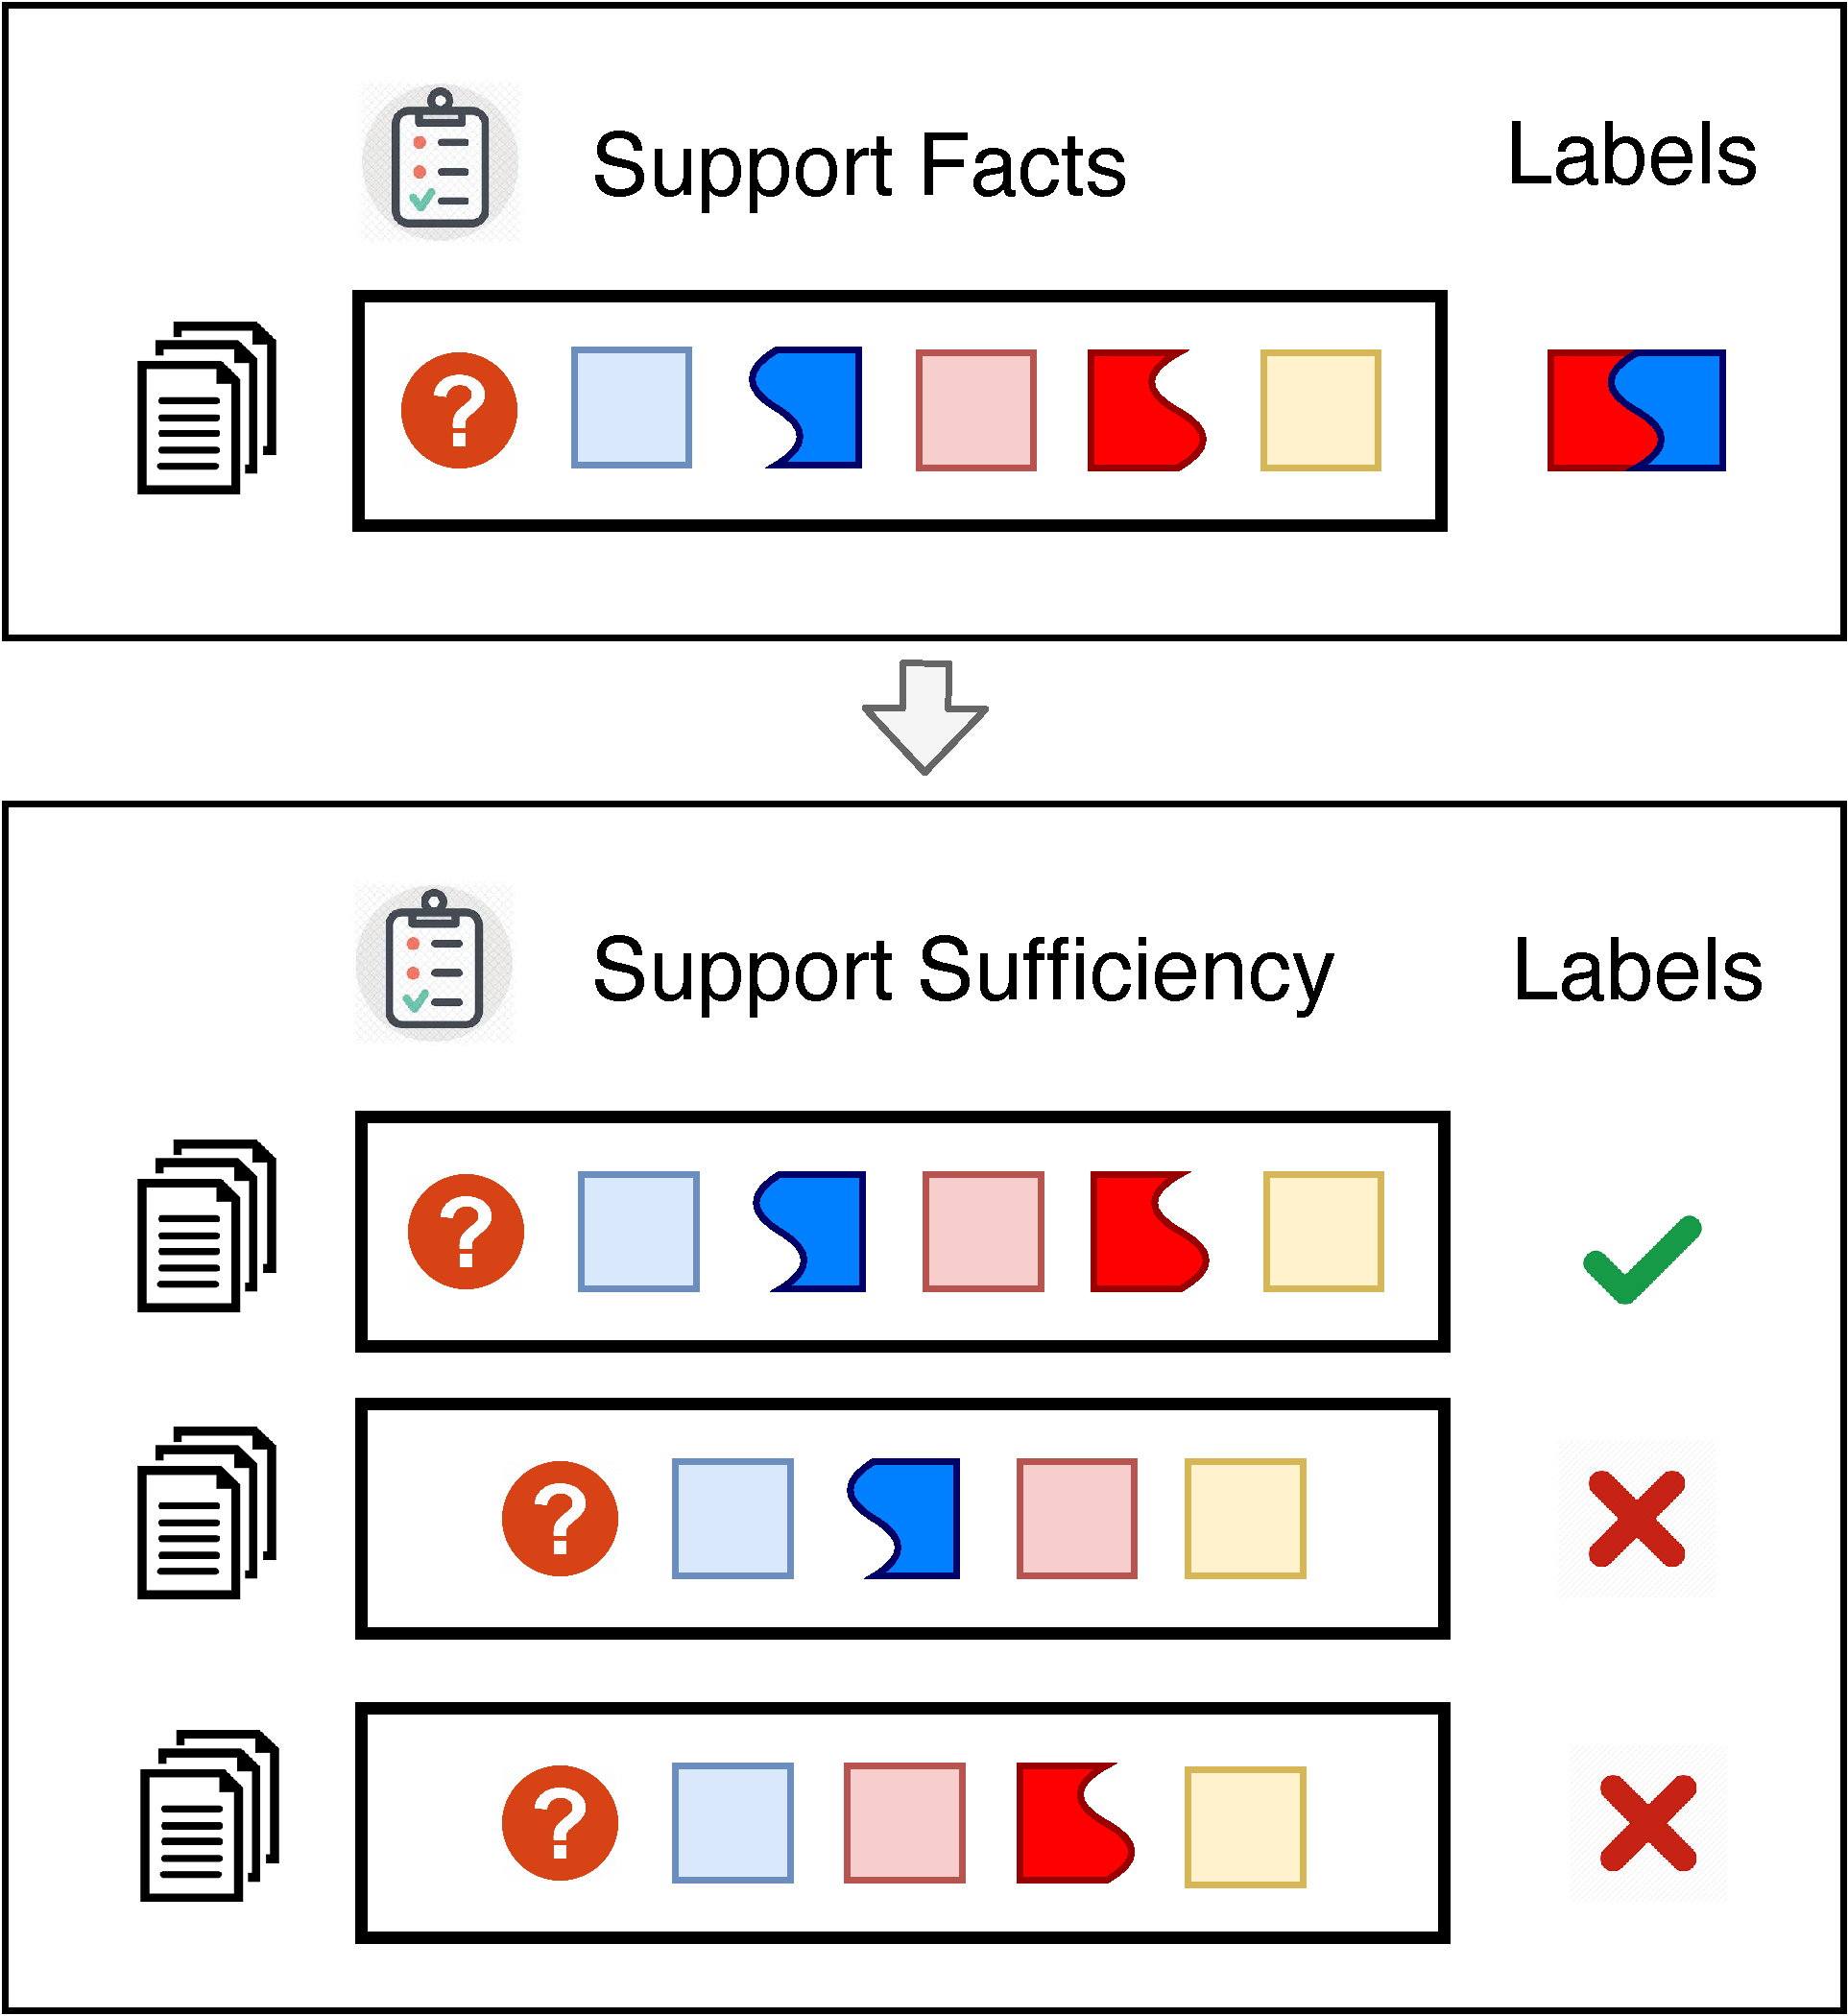
\includegraphics[width=0.35\textwidth]{images/transformation-v3}
	\caption{TODO: Explain why the support sufficiency prediction is harder than support location.}
	\label{fig:intro}
\end{figure}

%a subset of facts in the input context, i.e., given some $C^{\prime} \subseteq C$, test if $C^{\prime}$ contains {\em all} the supporting facts that necessary for answering the question.

%contains \it{all} the sufficient\harsh{supporting?} facts $F_s$ \harsh{sufficient} to support the correct answer. 

%We assume that the information in $F_s$ is not duplicated elsewhere in $C$. \harsh{Here, I think (i) we can say that task to test from some context $C$ itself. We use $C^{\prime} \subseteq C$ just to balance out the number of facts in positive and negative examples, but that's an implementation/method detail that we are anyway explaining later. (ii) I think if we say, "test if C contains all supporting facts", it won't be clear that it's all vs none, all vs partial or we annotate examples like Squad2. I think we need something that highlights this all vs partial check to separate what we are doing from general notion of unanswerable questions in Squad2 and others.}

\nb{Harsh, I am highly confident that I am wrong in what I have written below. Can you fix it?}

We first create sufficient context instances of a fixed size using all the sufficient facts $F_s$ and different subsets of other facts in $F_c$.
We create examples of insufficient contexts as follows. First, we create multiple (proper) subsets of the supporting facts. For each such proper subset $F_p$ we add some other facts from the original input context to create an insufficient context.\footnote{This process creates multiple negative instances for each positive instance. During training we balance the instances through under sampling but during test time we test on all negative examples since a model must be robust to all insufficient contexts.} We ensure that the size of the contexts is the same for both sufficient and insufficient cases.
\nb{Say something here that explains the equation below.}
\begin{itemize}[noitemsep]
    \item $(Q, F_s + F_d'; L_C=1)$
    \item $(Q, F_p + F_q + F_d'; L_C=0)$
\end{itemize}

A model passes the sufficiency test if and only if it is able to identify the sufficient and insufficient contexts in all cases. 

All of these \mfr tests, including sufficiency, can be hacked by \nmfr as long as there are artifacts and biases in the datasets. It turns out that we can measure how much models can score on these tests using \nmfr by devising probes 

%However, as we discuss in the next section, sufficiency test is significantly more difficult to hack in practice than the finding answer and supporting fact tests. Next, we show how we can turn these tests into probes for measuring \nmfr.


%Like answer and supporting fact tests, this support sufficiency test can also be hacked by non-multi-fact reasoning, but as we will discuss in the next section, that in practice, it's significantly less cheatable.

%Suppose that $F_s$ is the exact set of supporting facts in $C$ i.e., there exists no other subset of $C$ that duplicates information present in $F_s$.

%Assume that $F_s$ is the only support for humans to arrive at the answer for {\it Q} in {\it C}, i.e., the information crucial to arrive at the answer in any of the supporting facts $F_s$ is not duplicated in $F_d$. Under such a setting, we can automatically create instances where sufficient support is absent in the context and we can require the model to distinguish such instances with insufficient support from instances with sufficient support. Consider $F_p$ to be some proper subset of $F_s$. The context $F_p + F_d$ does not have sufficient support to answer the question, whereas $F_s + F_d$ has. So we can require the model to predict a binary class of sufficiency separating these two types of instances. Of course, we also need to make sure we don't introduce new biases making this classification task trivial.

\eat{
\tk{Possibly getting into the details after this. Doesn't seem necessary at this point}\harsh{Note that this is the only place we are introducing + describing our sufficiency based transform. It's not described anywhere else. The later section talks about: given this sufficiency based predictable property how can it be hacked.}
%Concretely, consider $|F_s| = n$ and $|F_d| = m$ with $m>n$. We randomly sample $n-1$ facts from $F_d$ to form $F_r$ and call the remaining facts in $F_d$ as $F_d'$. We create a sufficient support context with $F_s + F_d'$. And for each proper subset $F_p$, we sample $n-k$ examples from $F_r$ to form $F_q$ and create insufficient support context with $F_p + F_q + F_d'$. Note that $|F_s+F_d'| = |F_p + F_q + F_d'|$. Taking $L_c$ as a label for sufficient support present or not, for $F_p \subset F_s$, we construct the following examples:

\begin{itemize}[noitemsep]
    \item $(Q, F_s + F_d'; L_C=1)$
    \item $(Q, F_p + F_q + F_d'; L_C=0)$
\end{itemize}

We do this for all proper subsets of $F_s$ and the model gets a point if it exactly identifies the sufficiency classification for \textit{all} variations generated from independent of each other. \harsh{IMP:} The model needs to make decision on each variation independent of others. Note that for all the variations the positive example is the same. At training time, we sample only one negative example for each each question to balance the dataset and at test time, we test it on all subset variations.

In practice, we propose a sufficiency-based transform that requires the model to predict all the three properties - answer, supporting facts and support sufficiency. We care about answer and relevance prediction only in the positive examples of sufficiency. The model gets a point if it gets a point in all of the individual properties.

The insufficiency prediction can be compared unanswerability of questions in SQUAD 2.0 which has been used to reduce reliance of models on superficial surface-level cues as pervasive in SQUAD 1.0. Importantly though, we propose an automatic way of constructing unanswerable questions and show it's link with multi-fact reasoning. Like answer and supporting fact properties, the support sufficiency is also cheatable by non-multi-fact reasoning, but we will discuss in the next section, that in practice, it's significantly less cheatable.


}

% \harsh{It's better to use "characterizing" instead of "defining" mf reasoning, given we know even if model is correctly predicting all the desired properties, it still doesn't imply good (multi-hop) "reasoning".}

% V1: 
% It is difficult to define \textit{what is good reasoning over text} in a quantifiable way given that we don't have a good understanding of how humans reason\cite{gardner2019making}. But we can characterize a good reasoning entity (model or human) to have an ability to answer a question in a QA task. This characteristic is although not a sufficient condition of good reasoning, is surely a necessary one. Like-wise it's also difficult to define \textit{what is good multi-hop reasoning in a quantifiable way}. But we can characterize a good multi-hop reasoning entity (model or human) to have an ability to predict certain attributes about the multi-hop solution that it is intended to take. One of such attributes that have been widely used in multi-hop reasoning research is identification of supporting (relevant) facts. Again, this characteristic is not a sufficient condition of good multi-hop reasoning, but is surely a necessary one.

% V2:
\eat{
Textual multi-fact reasoning can broadly be defined as the ability of an entity (human or machine) to aggregate and synthesize together information from different textual facts in a ``meaningful" way that generalizes to novel combinations of textual facts\tk{We don't seem to talk much about how this ``meaningful'' combination leads to generalization, I think. It might be okay to drop ``that generalizes...'' part}. One way of estimating the (multi-fact) reasoning abilities of a system is through the task of (multi-fact) question answering posed in given textual context. 

Concretely, we assume a multi-fact question answering dataset, where question {\it Q} in a dataset {\it D} has an associated context {\it C} and the correct answer is {\it A}. The context {\it C} is a set of facts $C = F_s + F_d$, where annotated $F_s$ is a set of supporting facts and $F_d$ is a set of distractor facts\footnote{A \textit{fact} is any continuous text like paragraph or sentence.}. We assume a human can answer the question by synthesizing at least some information from \textit{all} the supporting facts in a known subset of facts. \tk{Rather than tying this too annotations, which can be noisy, what if we instead talk in terms of some set of supporting facts? E.g. C is a set of facts that contains a set of supporting facts needed to answer the question, $F_s$ (and the rest are considered distractor facts $F_d$)}


Given this setup, we can expect a good reasoning entity (model or human) to have an ability to be able to predict the answer to the questions, and also predict certain attributes for an arbitrary question about the multi-fact solution that it is intended to take to arrive at the answer from the question \tk{Was hard to parse. Maybe ``Given this setup, we can expect a good reasoning entity (model or human) to be able to predict the answer as well as certain properties indicating the solution to arrive at the answer for any question.''.}. We call everything we expect models to predict on a QA instance a predictable property of the instance.

Two such properties which have been used in (multi-fact) QA research are: \\

\noindent \textbf{Answer Prediction:} Given instance input {\it (Q, C)}, the model should be able to predict associated answer {\it A}. Using $P_a$ to denote the answer property label, the input output behavior we expect is $(Q, C) \Rightarrow P_a{=}A$. The system gets a point on given question-context pair for answer property only if it predicts the answer exactly correctly. \\

\noindent \textbf{Supporting Facts Prediction} Given instance input {\it (Q, C)}, the model should be able to predict associated set of supporting facts $F_s$. Using $P_s$ to denote the supporting facts property label, the input output behavior we expect is $(Q, C) \Rightarrow P_s{=}F_s$. The system gets a point on given question-context pair for supporting facts property only if it predicts the whole set of supporting facts exactly correctly.

Although ability to predict such properties is a desirable one, it does not imply good reasoning owing to various biases and artifacts present in the dataset that pave shortcuts for models to predict the property correctly without the intended reasoning. \tk{We mention these biases/artifacts few times now. So a natural question would be: Shouldn't we try to remove these artifacts? Or does our transformation get rid of artifacts?}

The properties, answer and supporting facts are especially hackable because the model can assume that the answer and both the supporting facts are also present in the context. In this case, the support identification reduces to supporting \textit{facts} identification, where as long as models can identify (locate) the supporting facts, it gets a point. This means it does not need to know whether these supporting facts are sufficiently supporting the answer. 

To mitigate this problem, we propose to add another property which we call sufficiency prediction, in which the model needs to identify whether sufficient support is present in the context to arrive at the answer. Importantly, we show an automatic way of constructing such instances by leveraging the supporting facts from the multi-fact QA dataset. \\

\noindent \textbf{Support Sufficiency Prediction:} Assume that $F_s$ is the only support for humans to arrive at the answer for {\it Q} in {\it C}, i.e., the information crucial to arrive at the answer in any of the supporting facts $F_s$ is not duplicated in $F_d$. Under such a setting, we can automatically create instances where sufficient support is absent in the context and we can require the model to distinguish such instances with insufficient support from instances with sufficient support. Consider $F_p$ to be some proper subset of $F_s$. The context $F_p + F_d$ does not have sufficient support to answer the question, whereas $F_s + F_d$ has. So we can require the model to predict a binary class of sufficiency separating these two types of instances. Of course, we also need to make sure we don't introduce new biases making this classification task trivial.

\tk{Possibly getting into the details after this. Doesn't seem necessary at this point}\harsh{Note that this is the only place we are introducing + describing our sufficiency based transform. It's not described anywhere else. The later section talks about: given this sufficiency based predictable property how can it be hacked.}
Concretely, consider $|F_s| = n$ and $|F_d| = m$ with $m>n$. We randomly sample $n-1$ facts from $F_d$ to form $F_r$ and call the remaining facts in $F_d$ as $F_d'$. We create a sufficient support context with $F_s + F_d'$. And for each proper subset $F_p$, we sample $n-k$ examples from $F_r$ to form $F_q$ and create insufficient support context with $F_p + F_q + F_d'$. Note that $|F_s+F_d'| = |F_p + F_q + F_d'|$. Taking $L_c$ as a label for sufficient support present or not, for $F_p \subset F_s$, we construct the following examples:

\begin{itemize}[noitemsep]
    \item $(Q, F_s + F_d'; L_C=1)$
    \item $(Q, F_p + F_q + F_d'; L_C=0)$
\end{itemize}

We do this for all proper subsets of $F_s$ and the model gets a point if it exactly identifies the sufficiency classification for \textit{all} variations generated from independent of each other. \harsh{IMP:} The model needs to make decision on each variation independent of others. Note that for all the variations the positive example is the same. At training time, we sample only one negative example for each each question to balance the dataset and at test time, we test it on all subset variations.

In practice, we propose a sufficiency-based transform that requires the model to predict all the three properties - answer, supporting facts and support sufficiency. We care about answer and relevance prediction only in the positive examples of sufficiency. The model gets a point if it gets a point in all of the individual properties.

The insufficiency prediction can be compared unanswerability of questions in SQUAD 2.0 which has been used to reduce reliance of models on superficial surface-level cues as pervasive in SQUAD 1.0. Importantly though, we propose an automatic way of constructing unanswerable questions and show it's link with multi-fact reasoning. Like answer and supporting fact properties, the support sufficiency is also cheatable by non-multi-fact reasoning, but we will discuss in the next section, that in practice, it's significantly less cheatable.

}
% Like answer and relevance prediction, sufficiency prediction is also not a a sufficient condition for good (multi-hop) reasoning, but is surely a necessary one. In the next section, we show how to capture the extent of information present in the dataset that paves shortcut to correct predictions.


% On such a dataset, a good reasoning model should be able to predict whether the information present in it is sufficient to answer the question or not. To automatically create positive and negative examples of binary classification of sufficiency we leverage the supporting facts annotation. The dataset only has positive examples of sufficiency. But for each positive example, we can create several negative example where the only supporting facts present in the context are proper subsets and not full set of annotated supporting facts. We further need to balance out the total number of facts in sufficient and insufficient examples to not inject this new bias that could make binary classification trivial.




% On such annotated dataset, a good reasoning entity (machine or human) should be able to predict the answer to arbitrary questions on the text. Furthermore, we can also expect a good multi-hop reasoning entity (model or human) to have an ability to predict certain attributes for an arbitrary question about the multi-hop solution that it is intended to take to arrive at the answer from the question. One such attribute that has been widely used in multi-hop reasoning research is identification of supporting (relevant) \ashish{This migth be the place to clarify: when datasets guarantee there is always full support present, \emph{support identification} reduces to the generally simpler task of \emph{relevance identification}, which we show is quite susceptible to NMF reasoning. However, when full support isn't guaranteed to be present, identifying whether full support is present is a strictly harder task than relevance identification, and a better assessment of multihop reasoning} facts which the system is intended to use and compose information from to arrive at the answer.

% The predictability of answer and relevance is not a sufficient condition for good (multi-hop) reasoning, but is surely a necessary one. This is because of various kinds of shortcuts exploitable by the model on the dataset task to evade the intended reasoning. Consider the example question \textit{"Which city was Facebook launched in?"} with two supporting facts (i)\textit{"Facebook was launched in Harvard."} and (ii)\textit{"Harvard is in \textbf{Cambridge} city."}, and some distracting facts. The intended reasoning here is to compose the information from the two supporting facts "meaningfully" to arrive at the answer and relevance predictions. However, depending on how the distracting the distracting facts are, a model can get both answer and relevance predictions right without any meaningful composition of facts that can generalize. For example, if there is no other mention of \textit{city} apart of supporting fact (ii), then answer and that supporting fact are easy to identify just through the question without any supporting fact composition. Similarly, if the supporting fact (i) is the only fact that has high overlap with the question, that relevant fact can also be identified through question and without any supporting fact composition. So both answer and (both) relevant facts can be identified without any meaningful supporting fact composition. The entity type matching and word overlap in the example here is just to give an intuitive notion of cheating. But the current generation of powerful pre-trained models are able to go far beyond such checks, allowing all of answer and relevance to be identified without any meaningful composition. This information can be misused by the model to "hack" the correct answer and relevance predictions.

% Such composition-less or interaction-less reasoning over supporting facts to hack answer and relevance prediction is fairly easily possible because models can assume that both the answer and both relevant facts are always present in the context. Removing this assumption, can mitigate such interaction-less reasoning (shortcuts) to a large extent. In the example above, we require the model to determine whether sufficient information is present in the context to answer the question or not based on whether \textit{both} supporting facts are present or not in the context, and if it is then further predict the answer and relevant facts. We will show in the later section that sufficiency prediction can also be hacked by interaction-less reasoning, but to a significantly lesser degree.

% We not that trivial AND can solve it if ....
% Model can no more make predictions in each part independent of other part. It has to do x.
% Most of the reasoning shortcuts in existing datasets arise due to the fact that the system can assume that the answer is guaranteed to exist in the given passage. Removing this assumption and
% requiring the system to identify whether the question is even answerable from the passage can prevent such shortcuts.

% One way of mitigating the problem is by requiring the models to determine the difference between the presence of both supporting facts and just one supporting fact in the set of facts as its context. The model now cannot do X
% One way of mitigating the problem is by requiring the models to separate out the difference of 

% TODO: Explain with example why answer and relevance both are fairly easily hackable in a way that directly motivates sufficiency prediction to mitigate this problem.

